    % Parabel
    \begin{subfigure}[c]{0.33\textwidth}
    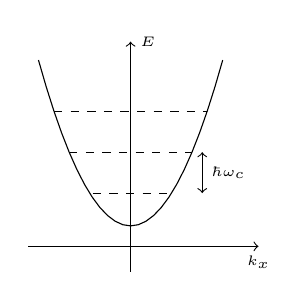
\begin{tikzpicture}[scale=1.3]
        % Koordinatensystem
        \draw [->] (0,-0.25) -- (0,2);
        \draw [->] (-1,0) -- (1.25,0);
        \draw (0,2) node[anchor=west] {\tiny $E$};
        \draw (1.25,0) node[anchor=north] {\tiny $k_x$};
        % Funktion
        \draw[domain=-0.9:0.9] plot ({\x}, {2*\x*\x+0.2});
        % Beschriftung
        \draw [dashed] (-0.37,0.52) -- (0.4,0.52);
        \draw [dashed] (-0.6, 0.92) -- (0.6,0.92);
        \draw [dashed] (-0.748,1.32) --(0.748,1.32);
        \draw [<->] (0.7,0.52) -- (0.7,0.92);
        \draw (0.7,0.72) node[anchor=west] {\tiny $\hbar \omega_c$};
    \end{tikzpicture}
    \subcaption{Diskrete Zustände bei Energiewerten der Landauniveaus}
    \end{subfigure}
    % Kreise
    \begin{subfigure}[c]{0.33\textwidth}
    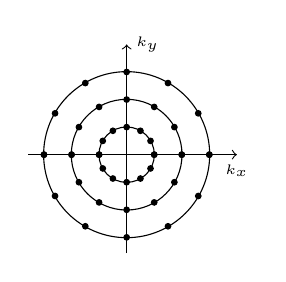
\begin{tikzpicture}
        % Koordinatensystem
        \draw [->] (-1.25,0) -- (1.4,0);
        \draw [->] (0,-1.25) -- (0,1.4);
        \draw (1.4,0) node[anchor=north] {\tiny $k_x$};
        \draw (0,1.4) node[anchor=west] {\tiny $k_y$};
        % Kreise
        \draw (0,0) circle (10pt);
        \draw (0,0) circle (20pt);
        \draw (0,0) circle (30pt);
        % Zustände
        \foreach \r in {0.35,0.7,1.05}{
            \foreach \x/\y in {0/1,1/0,-1/0,
                               0.8660254037844387/0.49999999999999994,% pi/6
                               0.49999999999999994/0.8660254037844387,% pi/3
                               -0.4999999999999998/0.8660254037844387,
                               -0.8660254037844387/0.49999999999999994
            }{
                \pgfmathsetmacro{\test}{1-(\x*\x)}
                \draw [fill] (\r*\x,\r*\y) circle (1pt);
                \draw [fill] (\r*\x,-\r*\y) circle (1pt);
            }
        }
    \end{tikzpicture}
    \subcaption{Zustände kondensieren auf Kreislinien}
    \end{subfigure}
    % Energiediagramm
    \begin{subfigure}[c]{0.3\textwidth}
        \begin{tikzpicture}[scale=1.15]
            \begin{axis}[xmin=0,xmax=4.5,ymax=1.2,
                xlabel={$E$},ylabel={$D(E)$},
                x label style={at={(current axis.right of origin)},
                               anchor=north,below=-0mm,left=-0.5mm},
                y label style={at={(current axis.above origin)},
                               anchor=south,below=-2mm},
                ticks=none]
                \addplot[blue] coordinates {(1,0)(1.1,1)(1.2,0)} ;
                \addplot[blue] coordinates {(2,0)(2.1,1)(2.2,0)} ;
                \addplot[blue] coordinates {(3,0)(3.1,1)(3.2,0)} ;
            \end{axis}
            \draw [<->] (0.8,0.95) -- (1.1,0.95);
            \draw (0.95,0.95) node[anchor=south] {\tiny $\hbar \omega_c$};
        \end{tikzpicture}
    \subcaption{Zustandsdichte spaltet in diskrete Landauniveaus auf}
    \end{subfigure}
